\documentclass[10pt]{article}
\usepackage[T1]{fontenc}
\usepackage[
    papersize={9in, 12in}, left=0.5in, right=0.75in, top=0.75in]{geometry}
\usepackage{array, booktabs, fontspec, nopageno, xfrac, xltxtra, xunicode}
\usepackage[
    %activate={true,nocompatibility},tracking=true,kerning=true,spacing=true,
    final, factor=1100, stretch=10, shrink=10]{microtype}
\setmainfont{Adobe Garamond Pro}
\begin{document}

\begin{center}

{\huge \textsc{Playing Techniques}}

\end{center}

\vspace*{1\baselineskip}

\newcolumntype{V}{>{\centering\arraybackslash} m{2cm} }
\newcolumntype{W}{>{\centering\arraybackslash} m{8cm} }
\renewcommand{\arraystretch}{2.5}

\begin{tabular}[t]{Vm{8cm}}
\textbf{XFB}
    & 
    ``extremely fast bow'': very pronounced flautando;
    play with generous amounts of bow lightly skimming the string;
    resulting color almost `fluorescent';
    prolong the color with irregular retakes of the bow as necessary;
    only occurs at quiet dynamics.
    \\

\textbf{spazz.}
    &
    spazzolato:
    sweep bow repeatedly up and down string in $\sfrac{1}{2}$ clt position;
    also `spz.'
    \\

\end{tabular}

\vspace*{5\baselineskip}

\begin{tabular}[t]{Wm{8cm}}
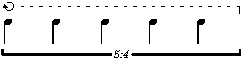
\includegraphics{../_assets/circle.pdf}
    &
    circle bowing;
    one complete circle per duration;
    five circles shown here.
    \\[1.75cm]
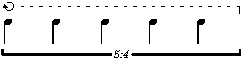
\includegraphics{../_assets/circle.pdf}
    &
    circle bowing.
    \\[1.75cm]
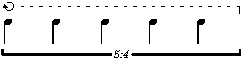
\includegraphics{../_assets/circle.pdf}
    &
    circle bowing;
    one complete circle per duration;
    five circles shown here;
    even more explanatory text;
    several additional words.
    \\ 
\end{tabular}

\vspace*{2.5\baselineskip}

\begin{center}

{\huge \textsc{String Contact Points}}

\end{center}

\begin{tabular}[t]{Vm{8cm}}

\textbf{T} & tasto
    \\

\textbf{P} & ponticello
    \\

\textbf{DZ}
    &
    ``dead zone'': last 1 cm of string closest to bridge (but not yet touching
    bridge); pitch almost (but not completely) effaced.
    \\

\textbf{OB}
    &
    ``on bridge'': bow directly on wood of bridge;
    pitch completely effaced;
    resultant sound gives snowlike whitenoise.
    \\

\end{tabular}

\end{document}
